\chapter{Introduction}
Computer graphics is the task of taking a virtual description of a scene, composed of objects such as models and lights, and rendering that scene to an image. One of the core components involved with this is computing realistic lighting. Although light behavior is fairly well understood in the physical sense, accurately simulating this behavior is a heavy computational task. The goal in computer graphics, then, is how to efficiently approximate light behavior where there are time and resources constraints.

% TODO paragraph or subsection about raytracing/offline gi somewhere?

Of particular importance in computer graphics are real-time applications, where images, or frames, must be produced at an interactive speed, such as video games. Typically, the lower bound for this is considered 30 frames per second, or about 33 milliseconds per frame, and a target of 60 frames per second, or about 17 milliseconds per frame. To meet this goal, researchers and engineers have designed many algorithms and techniques.
% TODO reword
In this work, we implement and extend an algorithm to accomplish fast and accurate lighting for fully dynamic scenes. An example of our global illumination algorithm is shown in Figure~\ref{fig:introduction_gi}.

% TODO seems like a good thing to note (it's very engineer-y)
It is important to keep in mind that most lighting algorithms have many tradeoffs and are adapted towards specific use cases. A complete lighting system may also combine many different lighting algorithms in order to achieve the desired balance between quality, performance, and ease of use.

\begin{figure}[h]
\centering
    \begin{subfigure}[t]{0.4\textwidth}
        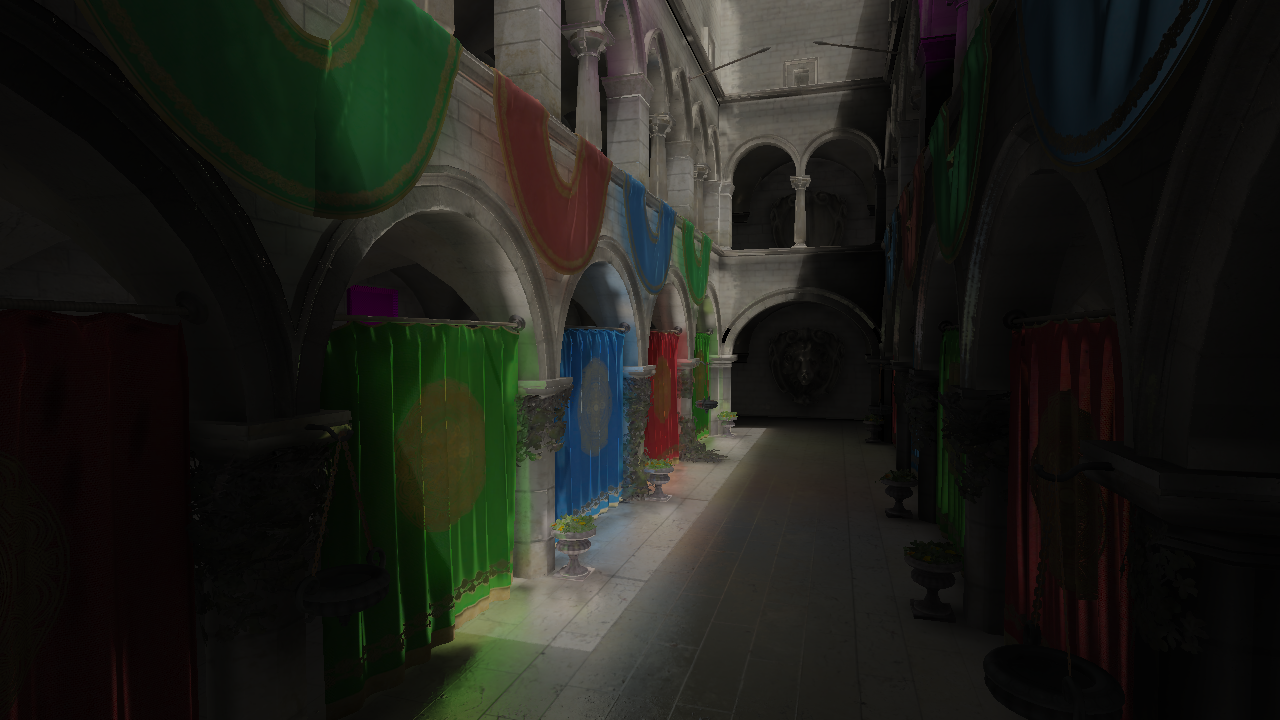
\includegraphics[width=\textwidth]{gi_on.png}
        \caption{Global illumination}
    \end{subfigure}
    ~
    \begin{subfigure}[t]{0.4\textwidth}
        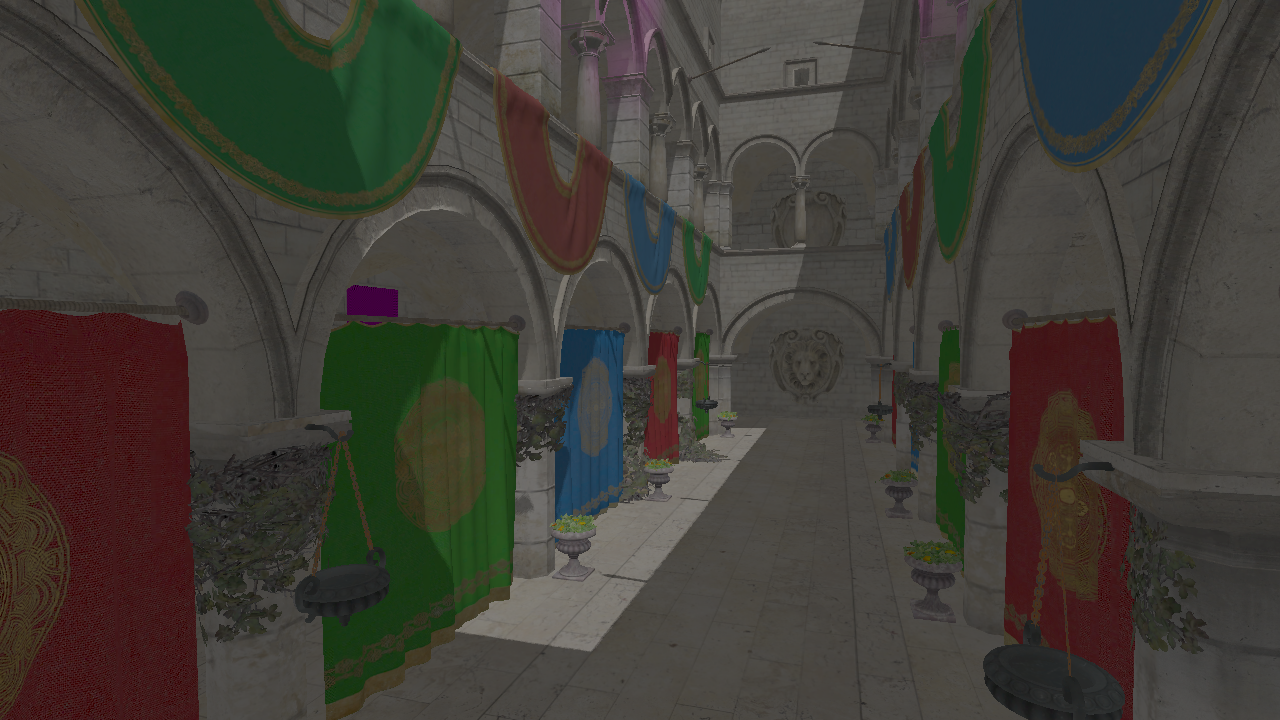
\includegraphics[width=\textwidth]{gi_off.png}
        \caption{No global illumination}
    \end{subfigure}
    \caption{A scene---describing information like light sources, materials, and geometry---is rendered by computing a color for each pixel of a screen. The image on the left is rendered with global illumination whereas the image on the right uses a constant ambient term for indirect lighting.}
    \label{fig:introduction_gi}
\end{figure}

\section{Real-Time Global Illumination}
In general, lighting at a given point is a combination of direct and indrect light. Direct light is light accumulated directly from a light source, whereas indirect light is the light that comes from other non-light sources in the scene (e.g.\ the light that has `bounced' off of objects in the scene).

% TODO ambient occlusion: footnote with citations for a few types (SSAO, HBAO, etc.)
% TODO cite specific sections of book howdo?
In the beginnings of computer graphics simple lighting models were used in order to maintain real-time performance. While the direct light was feasible to compute in real-time (albeit with limitations on number of lights and other optimizations), indirect lighting was often faked with a simple constant contribution. As hardware limitations and algorithms improved, more advanced techniques were developed and approximating the indirect light became more feasible. Two methods, ambient occlusion~\cite{bunnell2005dynamic,moller2008rtr} and baked lighting~\cite{Sloan:2002:PRT:566654.566612,moller2008rtr}, became standard ways of introducing simple global illumination, the term given to techniques that improved indirect lighting. However both these methods have drawbacks. Ambient occlusion, which approximates the effect of light occlusion by nearby objects, provides a great improvement over the constant ambient term used previously but does not accurately simulate the indirect light in its entirety. Thus it is only `partial' global illumination. Baked lighting involves pre-computing light behavior of a scene prior to runtime and then utilizing the precomputation to enable real-time realistic lighting. The drawback here is only static objects can have their light baked---any dynamic objects or lights in the scene are not accounted for.

% TODO reword
Full global illumination algorithms attempt to provide a complete approximation of indirect light. Some, like baked lighting, only work for static scenes. For our work, however, we are interested in dynamic global illumination. In other words, our goal is full global illumination that can be performed completely for each frame. Any changes in the scene---object movement, light movement or changes in intensity---will be accounted for.

For dynamic real-time global illumination, a common approach is to first construct a spatial representation of a scene's radiance (light information) and then use that representation to approximate the radiance at a given point in the scene. Popular methods that follow this approach are light propagation volumes~\cite{Kaplanyan:2010:CLP:1730804.1730821} and voxel cone tracing~\cite{crassin2011interactive} (see Related Works for more). Some challenges that arise from methods like these are issues with GPU memory consumption and achieving adequate lighting detail. % TODO expand on these problems more?

\section{Our Contribution}
% TODO should I put results here too?
The main contribution of this work is a complete implentation of computing global illumination based on voxel cone tracing with a focus on ease of use and speed while still producing high quality results. We hope this provides a competitive alternative to existing real-time global illumination systems that can be used for educational purposes.

 We also present an approach to scene voxelization using hardware tessellation and compare it with an approach utilizing hardware rasterization. We find similar performance to the raster approach approach but with promising results for perspective warped voxels. We also investigate possible methods of nonuniform voxelization.

%The novel contribution, voxel warping, is a way to handle large scenes in a memory efficient and simple way. The idea is to adjust the voxel density of the scene based on its distance from the camera, which allows a large scene to be represented without requiring large memory or performance overheads.

% TODO fact check and citations needed
Another important part of our contribution is that the implementation is open-source and cross platform (on Linux and Windows using modern OpenGL\footnote{macOS is not supported since Apple only supports up to OpenGL 4.1~\cite{appleopenglsupport}, whereas we require 4.5 (for features like compute shaders, direct state access, and image objects).}. Many graphics implementations are developed in the research or industrial space and are often not made available to the public for various reasons (e.g.\ copyright). Even implementations that are openly available often are tied to a specific game engine or other large codebase\footnote{For example, NVIDIA's VXGI is integrated into a custom branch of Unreal Engine 4 (distributed as a binary)~\cite{nvidiavxgi} and Light Propagation Volumes are implemented in CryEngine3~\cite{kaplanyan2009light}. The Godot engine~\cite{godotengine} is a notable exception here and, while part of a large codebase, is relatively small and is completely open source.}, making it difficult to understand or integrate into one's own project. Furthermore, many implementations utilize DirectX as their graphics API, which limits the implementation to Windows only. We hope that providing an easy to understand and cross platform implementation will help others learn more about voxel cone tracing and dynamic real-time global illumination.
